\documentclass[letterpaper, 12pt]{texMemo}
\usepackage[american]{babel}
\usepackage{graphicx}
\usepackage{caption}
\usepackage{float}
\usepackage[citestyle=apa,style=apa,backend=biber]{biblatex}
\captionsetup{justification = raggedright, singlelinecheck = false}
\DeclareLanguageMapping{american}{american-apa}
\addbibresource{bibliography.bib}
\memoto{Dr. William Hsu}
\memofrom{Blair Urish}
\memosubject{Sample of visual aids for literature review regarding Internet of Things Security}
\memodate{\today}

\begin{document}
\maketitle
\begin{flushleft}
\subsection*{Introduction}
The purpose of this memo is to provide examples of two visual aids that will be used in the final report. The memo also provides justifications for the
inclusion of each of the visual aids.

\subsection*{Figure 1}
This figure identifies the three layers of the Internet of Things architecture. The figure provides the reader with examples of services that function at each layer and
the security measures those services may require. 

\begin{figure}[H]
	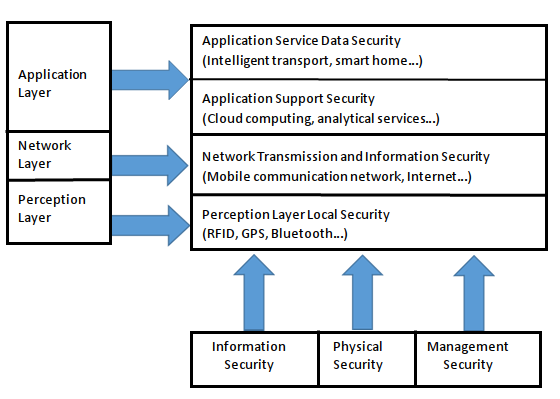
\includegraphics[width=\linewidth,height=10cm,keepaspectratio]{figure2_new.png}
	\caption{Internet of Things Architecture (adapted from \cite{Zhao6746513})}
	\label{fig:arch}
\end{figure}

\subsection*{Justification for Figure 1}
In the final report, the above layers will be used extensively when discussing security issues and standards. It is important that the reader has a good understanding of what types
of services are found at each layer of the Internet of Things architecture. The figure also provides a resource that the reader can refer back to as they read through the report.


\subsection*{Table 1}
This table shows the current communication standards that are used with Internet of Things (IoT) devices and the layer each standard is associated with. The table also provides
definitions for the various acronyms used to refer to these standards. When all of these standards are put together, they form a complete communication stack for an IoT
device. (\cite{Granjal7005393}).

\begin{table}[H]
\begin{tabular}{ | l | l | p{9cm} |}
\hline
Layer & Acronym & Full Name \\ \hline
Application & CoAP & Constrained Application Protocol \\ \hline
Network/routing & RPL & Routing Protocol for Low Power and Lossy Networks \\ \hline
Adaptation & 6LoWPAN & IPv6 over Low Power Personal Area Networks \\ \hline
MAC & n/a & IEEE 802.15.4, IEEE 802.15.4e \\ \hline
Physical & n/a & IEEE 802.15.4 \\ \hline
\end{tabular}
\caption{Internet of Things Communication Standards (adapted from \cite{Granjal7005393})}
\end{table}

\subsection*{Justification for Table 1}
In the final report, all of the standards in the above table will be discussed in detail. Having this table in the report will allow readers to quickly see what standards
will be addressed and what layer they apply to. It is also important
that the reader understands the meaning of the acronyms used for these standards because they will be used frequently in the final report. The reader can quickly refer back to the
table if they happen to forget the meaning of an acronym or what layer the standard is associated with. 

\newpage
\subsection*{References}
\fullcite{Zhao6746513}\\
~\newline
\fullcite{Granjal7005393}
\end{flushleft}
\end{document}
